\chapter{OnlyFacets exploratory search}
This chapter deals with the process of exploratory search and its implementation. We purpose a prototype named {\it OnlyFacet} search, as to fully evaluate the usability of our search prototype, we intend to remove key-word search bar. To begin with, an introductory example is presented and the functionality of the prototype graphical user interface (GUI) is explained.

\section{The user interface of {\it OnlyFacet} search}
The graphical user interface (Fig)is designed to comprise three main areas: the direct search results in the center of column, the {\it faceted filter} on the right, and the exploratory search navigation on the left. The search results include a timeline, which shows the automatically generated temporal segmentation of the results including highlighted segments indicating search hits. The facet filter allows to narrow down the search results based on graph search. 

\begin{figure}
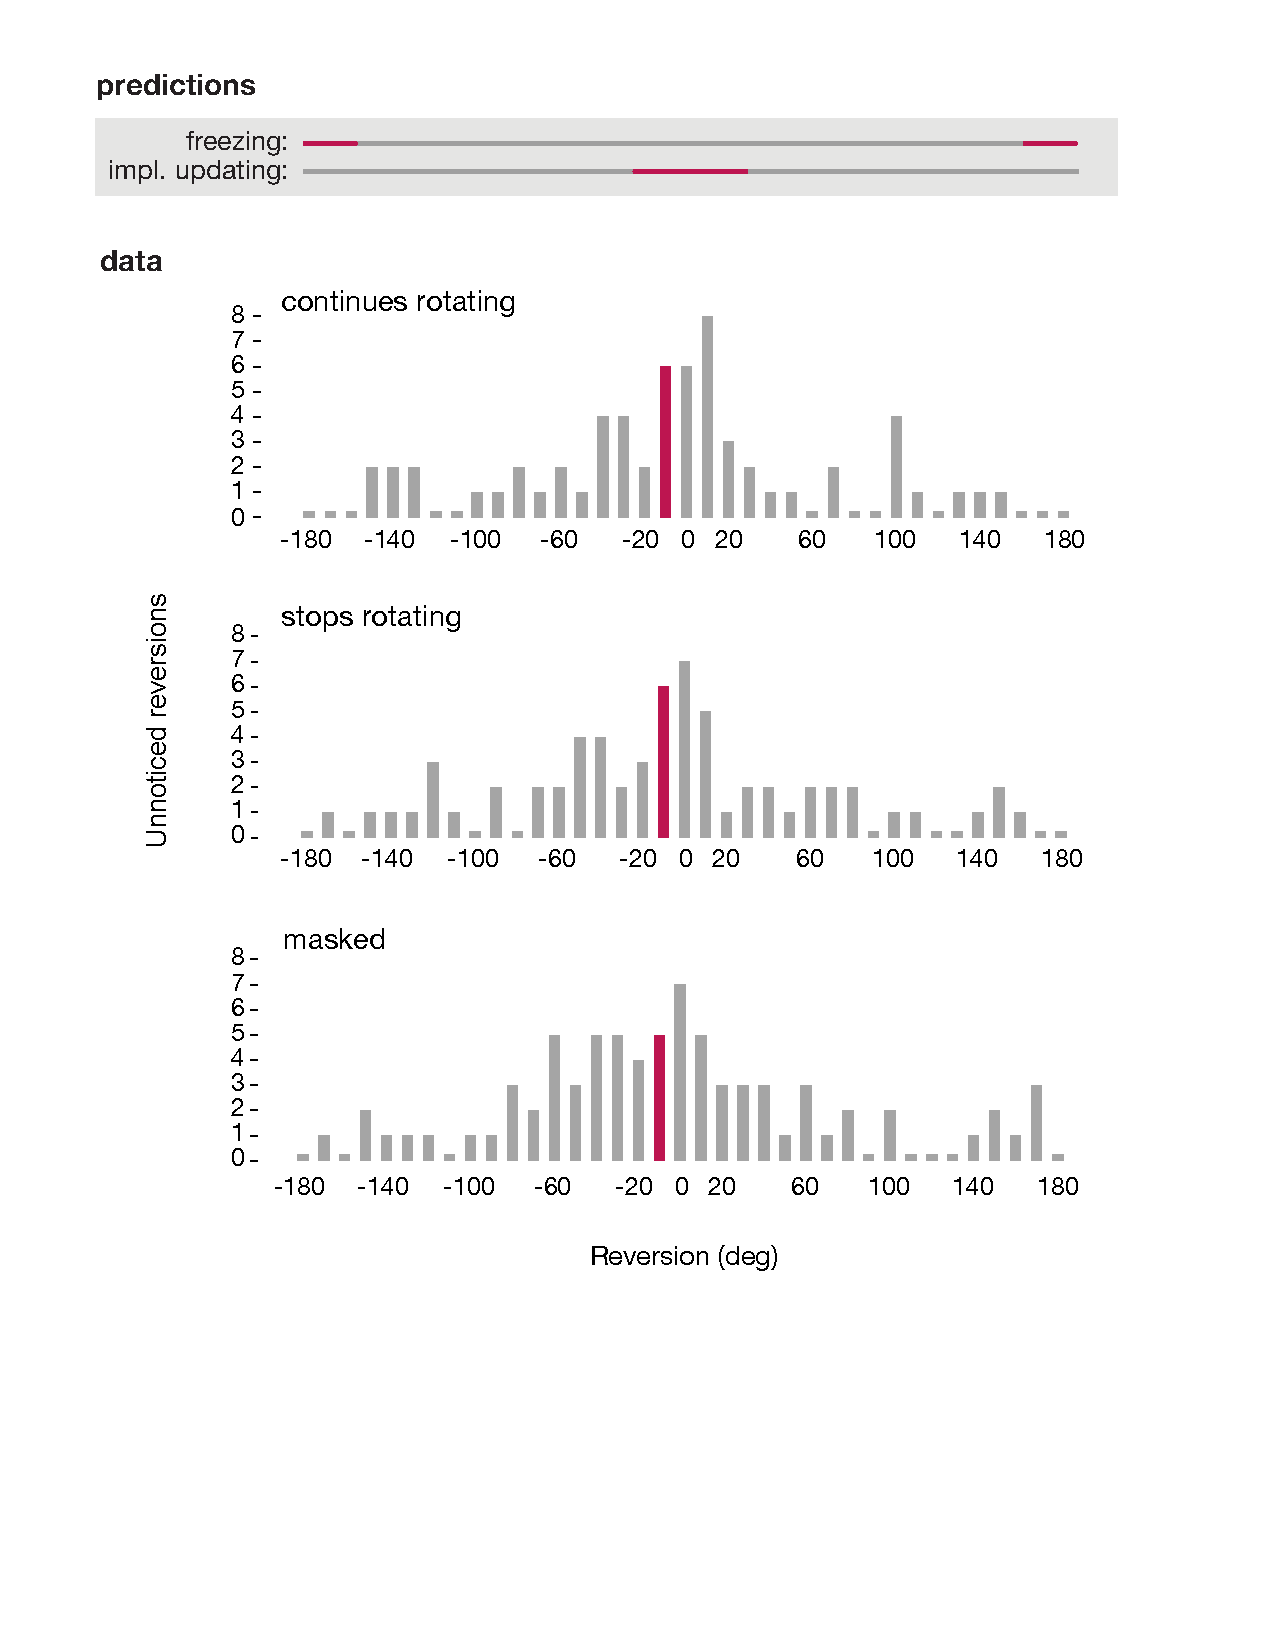
\includegraphics[width=\textwidth]{figures/fig2}
\caption[OnlyFacet Faceted Search.]{The {\it OnlyFacet} search GUI showing related entities for ``American Place''
\label{fig:myInlineFigure}}
\end{figure}

Faceted search aims to broaden the scope of search by suggesting related terms, concepts and resources. Our approach uses priority queue and data graph to support the search process by exposing additional information about indexed resources.

Figure 1 depicts the result of a query after the user clicking on the facets - restaurant and place. The exploratory search GUI suggests a list of related entities. When the user clicks multiple facets, the labels of the mapped entities grouped by their connecting properties. 

By clicking on, e.g. {\it 'Shia and Sunni'} in the faceted search GUI, a new search is issued and the GUI switches to the newly selected entity showing its related entities and properties (cf. Fig. 2). This supplementary information includes, as e. g., related places (birth place, work place, etc), predecessor and successor in the presidential office, or Barack Obama�s residence.

\begin{figure}
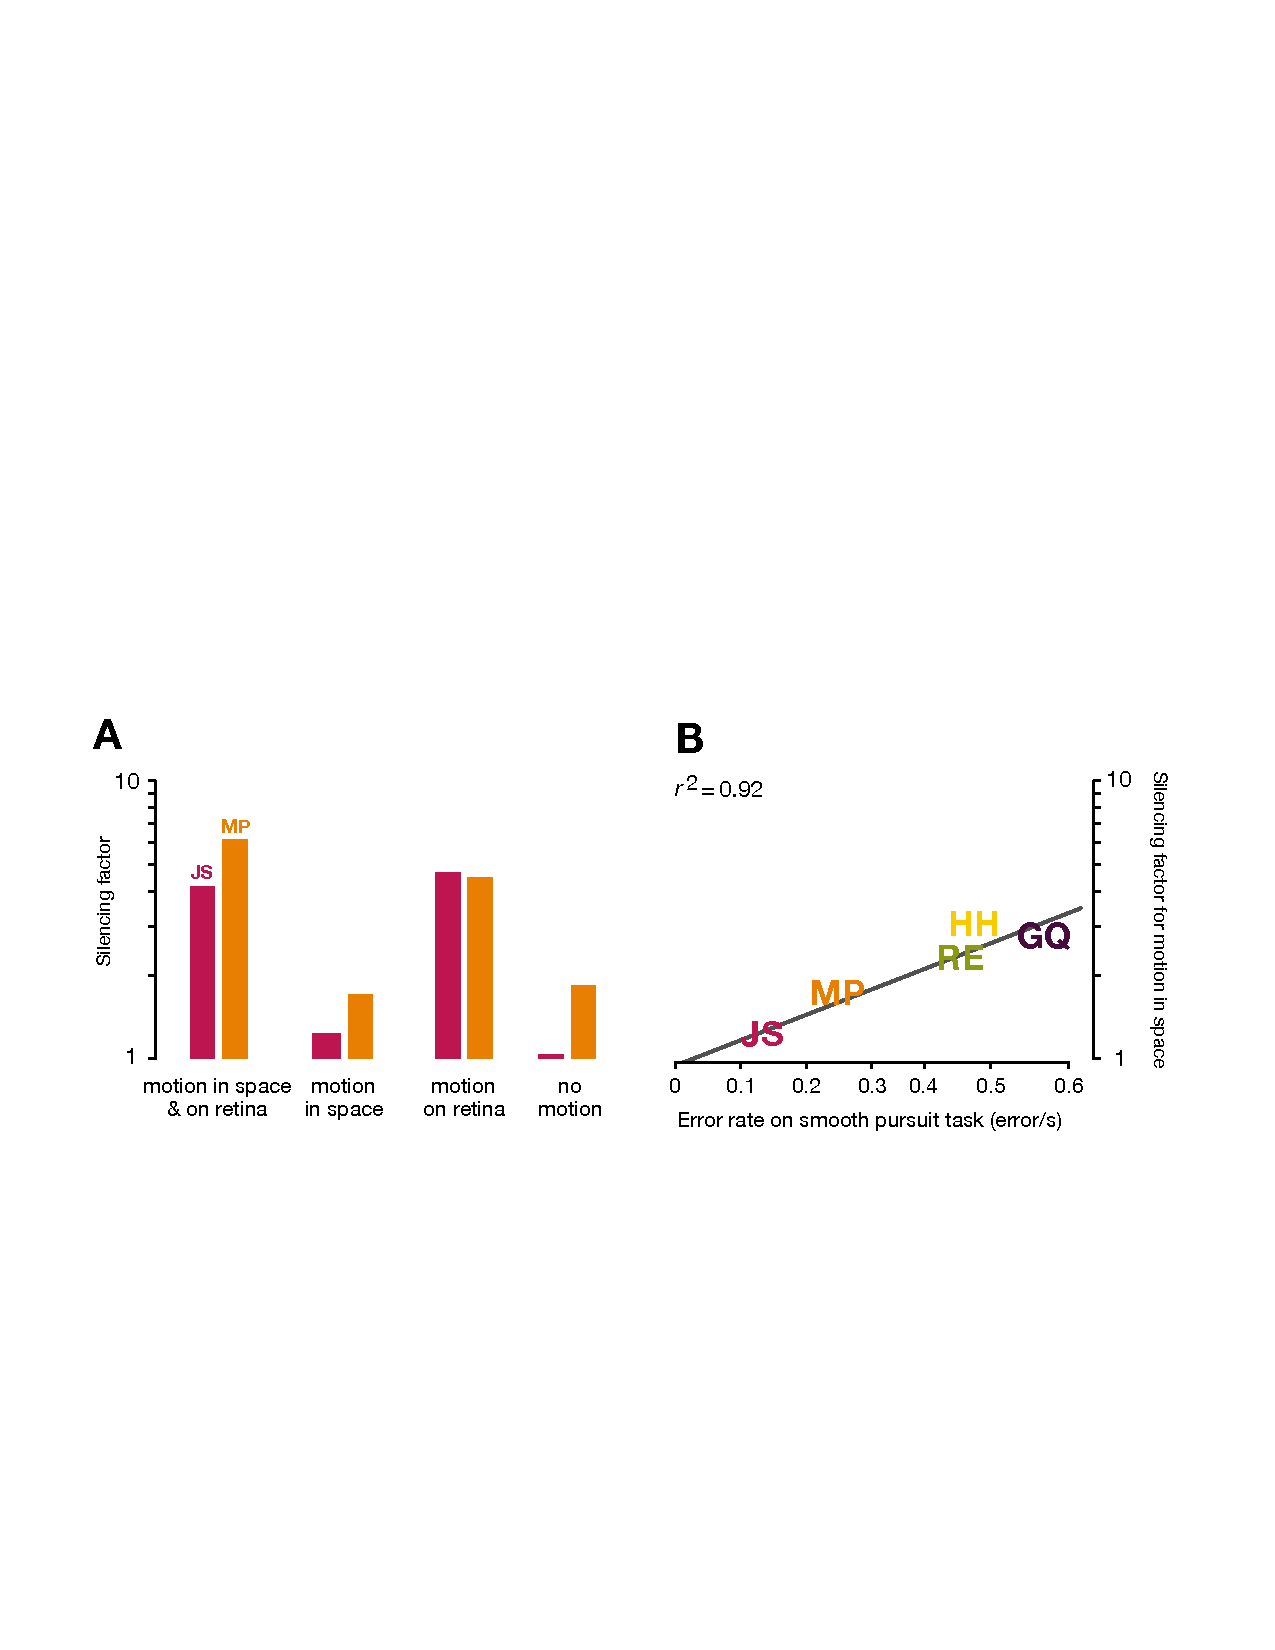
\includegraphics[width=\textwidth]{figures/fig3}
\caption[OnlyFacet Faceted Search.]{The {\it OnlyFacet} showing related entities for 'Shia and Sunni'
\label{fig:myInlineFigure}}
\end{figure}

To retain previous actions, a history list (4) provides links to previous searches. Optionally, the user may activate an additional preview of the search results evoked by a related entity when clicking on it (5). Moving the mouse pointer over these previews causes a popup to show brief information about the video resource (6).
